\section{Обзор современных нейронных сетей}
\label{sec:Chapter2} \index{Chapter2}

\subsection{Общие соображения}

Искуственная нейронная сеть --- математическая модель, а также её программное или
аппаратное воплощение, построенная по принципу организации биологических нейронных
сетей --- сетей нервных клеток живого организма. Этот принцип отражается в её
устройстве: нейронная сеть состоит из некольких слоёв, каждый из которых принимает
информацию с предыдущего, обрабатывает её каким-то образом, а  затем передаёт её
на следующий слой.

Благодаря новым исследованиям в этой области, нейронные сети нашли большое
количество применений в разных сферах жизни. В медицине они позволяют проводить
более точную диагностику заболеваний (например, онкологии), создавать портативные
устройтва для диагностики (например, для проведения ЭКГ). Они используются
для обработки больших данных в разных исследовательских областях, таких как
астрономия и геологоразведка. Также они упрощают жизнь в робототехнике и
автоматизации производства.

Рассмотрим наиболее популярные архитектуры нейронных сетей, их основные особенности.

\subsection{Обработка естественного языка}

Обработка естественного языка --- общее направление искусственного интеллекта и
математической лингвистики. Оно изучает проблемы компьютерного анализа и синтеза
текстов на естественных языках. Применительно к искусственному интеллекту анализ
означает понимание языка, а синтез --- генерацию грамотного текста. Одним из
подходов к решению данной задачи стала архитектура трансформер, представленная
компанией Google в 2017 году. Эта архитектура используется в переводчиках
(например, от компаний Яндекс и Google) и в чат-ботах (например, Chat GPT).
BERT, GPT-3, LLaMA --- модели, основывающиеся на архитектуре трансформер.

Многие из таких моделей можно скачать, после чего изучить их внутреннее
устройство. Нами была выбрана модель BERT. Не погружаясь в детали реализации
можно заметить, что подавляющее большиство операций в ней занимают
умножения матриц. По этой причине эта операция была выбрана для
дальнейшего исследования.

\subsection{Компьютерное зрение}

Компьютерное зрение --- теория и технология создания машин, которые могут
производить обнаружение, отслеживание и классификацию объектов. Распознавание
изображений может быть полезно в любой сфере, например, в сельском хозяйстве ---
для обнаружения болезни растений, в области безопасности --- для обнаружения
преступников и т.д.

Одно из наиболее популярных решений в этой области --- свёрточные нейронные
сети. Принцип их работы схож с работой зрительной коры головного мозга.
Основываются они на операции свёртки (конволюции). В функциональном анализе
она применяется к двум функциям и возвращает третью, соответствующую их
взаимной корреляции. Проще говоря, их можно интерпретировать как <<схожесть>>
двух функций.

В нейронных сетях свёртка применяется к изображениям, её схему можно увидеть
ниже. На часть изображения <<накладывается>> ядро, т.е. эта часть скалярно
умножается на ядро. Получившийся результат является каким-то признаком, он
записывается в результирующую матрицу --- матрицу выходных признаков
(output feature map). Стоит отметить, что общий случай свёркти несколько
сложнее, более подробно этот вопрос будет рассмотрен в соответствующей
главе.

\begin{figure}[h!]
    \centering
    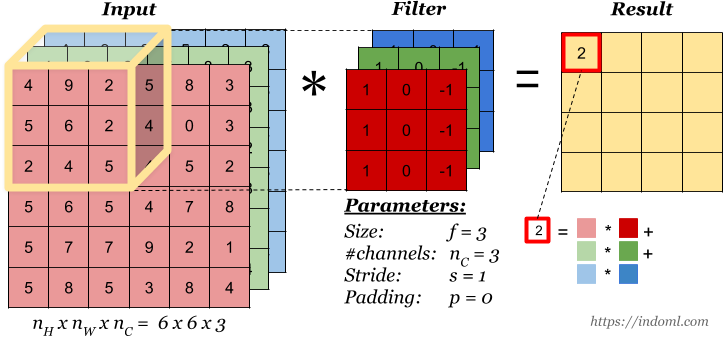
\includegraphics[scale=0.5]{Convolution.png}
    \caption{Операция свёркти для изображения с тремя цветами}
\end{figure}

Существует большое количество свёрточных нейронных сетей: LeNet-5, AlexNet,
VGG, GoogLeNet, ResNet, Inception. Нами была выбрана ResNet для дальнейшего
исследования. Она представлена несколькими вариантами, которые отличаются
количеством слоёв, а следовательно, точностью вычислений и размерами весов
модели. Модель с 18 слоями представлена на рисунке ниже. Как видно из
рисунка, в ней используются только операции свёркти. Но внутри них также
есть операции сложения и $Relu$, где

\[
    Relu(x) =
        \begin{cases*}
            x, ~ x \geqslant 0 \\
            0, ~ x < 0
        \end{cases*}
\]

\begin{figure}[h!]
    \centering
    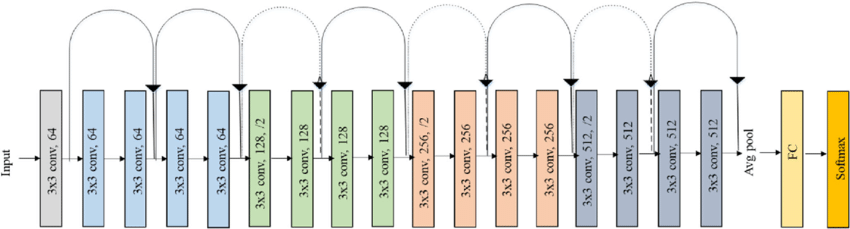
\includegraphics[scale=0.5]{ResNet18.png}
    \caption{Модель ResNet18}
\end{figure}

\newpage
